\problemname{Jammed Gym}

You are at the fitness centre to run through your exercise programme. You must
use the kinds of exercise machine in an order precisely dictated by the
programme, although there may be more than one instance of a machine.

You start at the centre of a unit circle around which the exercise stations are
arranged. You can walk directly between any two points in the circle, and you
may also visit the same point multiple times.
See Figure \ref{fig:jammedgym} below for an example.

\begin{figure}[h!]
  \centering
  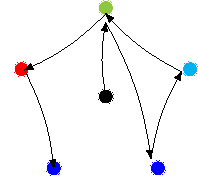
\includegraphics[width=0.4\textwidth]{fig}
  \caption{Illustration of Sample Input 1. Types of machine: $[1, 2, 4, 1, 3, 2]$}
  \label{fig:jammedgym}
\end{figure}

Exercise is an important and noble endeavour, but in today's busy world we must
strive for efficiency in everything we do. Find the most efficient way of
visiting exercise stations that matches the order given.

\section*{Input}
\begin{itemize}
\item The first line of input contains the number of exercises in the programme,
      $n$ ($1 \le n \le 100$).
\item The second line of input contains $n$ space-separated integers
      each denoting the type of an item on the programme $t$ ($1 \le t_i \le 100$).
      There will always be at least one station for each programme in this list.
\item The third line of input contains the number of stations,
      $m$ ($1 \le m \le 100$).
\item The fourth line of input contains $m$ space-separated integers
      each denoting the type of a station $q$ ($1 \le q_i \le 100$).
\end{itemize}

\section*{Output}

Output the minimum distance you will need to walk.
Your answer must be accurate to an absolute or relative error of $10^{-6}$.
